\hfill\break
\justifying
\textbf{DTW}
	\hfill\break
	\justifying
	\textit{Dynamic Time Warping}(DTW) es una técnica bien conocida para encontrar una alineación óptima entre 2 sequencias dependientes del tiempo(series de tiempo) dadas y bajo ciertas restricciones[14]. Este algoritmo es sumamente util para medir la similaridad entre dos secuencias temporales que no se alinean exactamente en el tiempo, velocidad o extensión[14]. Originalmente este algoritmo había sido utilizado para comparar patrones de habla en reconocimiento de habla automático, siendo aplicado en otros campos de forma exitosa para lidiar con deformaciones en el teimpo y diferentes velocidades.
	
	\hfill\break
	\justifying
	El objetivo de DTW es la comparación de 2 secuencias dependientes del tiempo \textit{X} y \textit{Y}, siendo series discretas, o más generalmente una secuencia de características muestreadas a puntos equidistantes en el tiempo.¸
	\begin{equation*}
		\begin{array}{cc}
			X = (x_1,x_2,...,x_N) & N \in \mathbb{N} \\
			Y = (x_1,x_2,...,x_M) & M \in \mathbb{N} \\
		\end{array}
	\end{equation*}
	
	\hfill\break
	\justifying
	Con un \textit{espacio de características} denotado por $\mathcal{F}$, la comparación de dos características diferentes se realiza mediante una \textit{medida de costo local}, también llamada \textit{medida de distancia local} definida por:
	\begin{equation*}
		c: \mathcal{F} \times \mathcal{F} \rightarrow \mathbb{R}_{\geq 0}
	\end{equation*}
	
	\hfill\break
	\justifying
	La implementación de la \textit{medida de distancia local} depende de la medida de distancia general definida, para el documento se implementa la distancia Euclidiana \textit{c} se define como: $c(x_i, y_j) = (x_i - y_j)^2$ donde $i \in [1:N]$ y $j \in [i:M]$, pero otro tipo de medidas de distancia local pueden utilizarse, como por ejemplo L1 o distancia \textit{Manhattan}.
	
	\hfill\break
	\justifying
	Tipicamente \textit{c(x,y)} es pequeña(bajo costo) si \textit{x} y \textit{y} son similares, de otra forma esta es alta. Evaluando el costo local medido para cada par de elementos de las secuencias \textit{X} y \textit{Y}, se obtiene la \textit{matriz de costo} $C \in \mathcal{R}^{N\times M}$ definida por $C(n,m):=c(x_n,y_m)$ entonces la meta es encontrar una alineación entre \textit{X} y \textit{Y} obteniendo el costo total mínimo.
	
	\hfill\break
	\justifying
	Formalmente un camino de deformación o \textit{warping path}, es una secuencia $p=(p_1,...,p_L)$ con $p_\ell = (n_\ell,m_\ell) \in [1:N]\times[1:M]$ para $\ell \in [1:L]$ satisfaciendo las siguientes 3 condiciones:
	\begin{enumerate}[label=(\roman*)]
		\item \textit{Condición límite}: $p_1=(1,1)$ y $p_\ell=(N,M)$
		\item \textit{Condición Monotonicidad}: $n_1\leq n_2\leq ... \leq n_L$ y $m_1\leq m_2\leq ... \leq m_L$
		\item \textit{Condición del tamaño del paso}: $p_{\ell + 1}-p_\ell\in{(1,0),(0,1),(1,1)}$ para $\ell \in [1:L-1]$
	\end{enumerate}
	
	\hfill\break
	\justifying
	Un \textit{(N,M)-warping path} $p=(p_1,...,p_L)$ define una alineación entre las secuencias \textit{X} y \textit{Y} al asignar el elemento $x_{n_\ell}$ al elemento $y_{m_\ell}$. Un ejemplo de la aplicación de las 3 condiciones durante la construcción del camino óptimo se observa en la Figura (3,\textit{a)}, donde utilizando la matriz de costo acumulado se marca una secuencia en color verde de las distancias óptimas satisfaciendo siempre las condiciones(i,ii,iii). 
	
	\hfill\break
	\begin{minipage}{\linewidth}
		\centering
		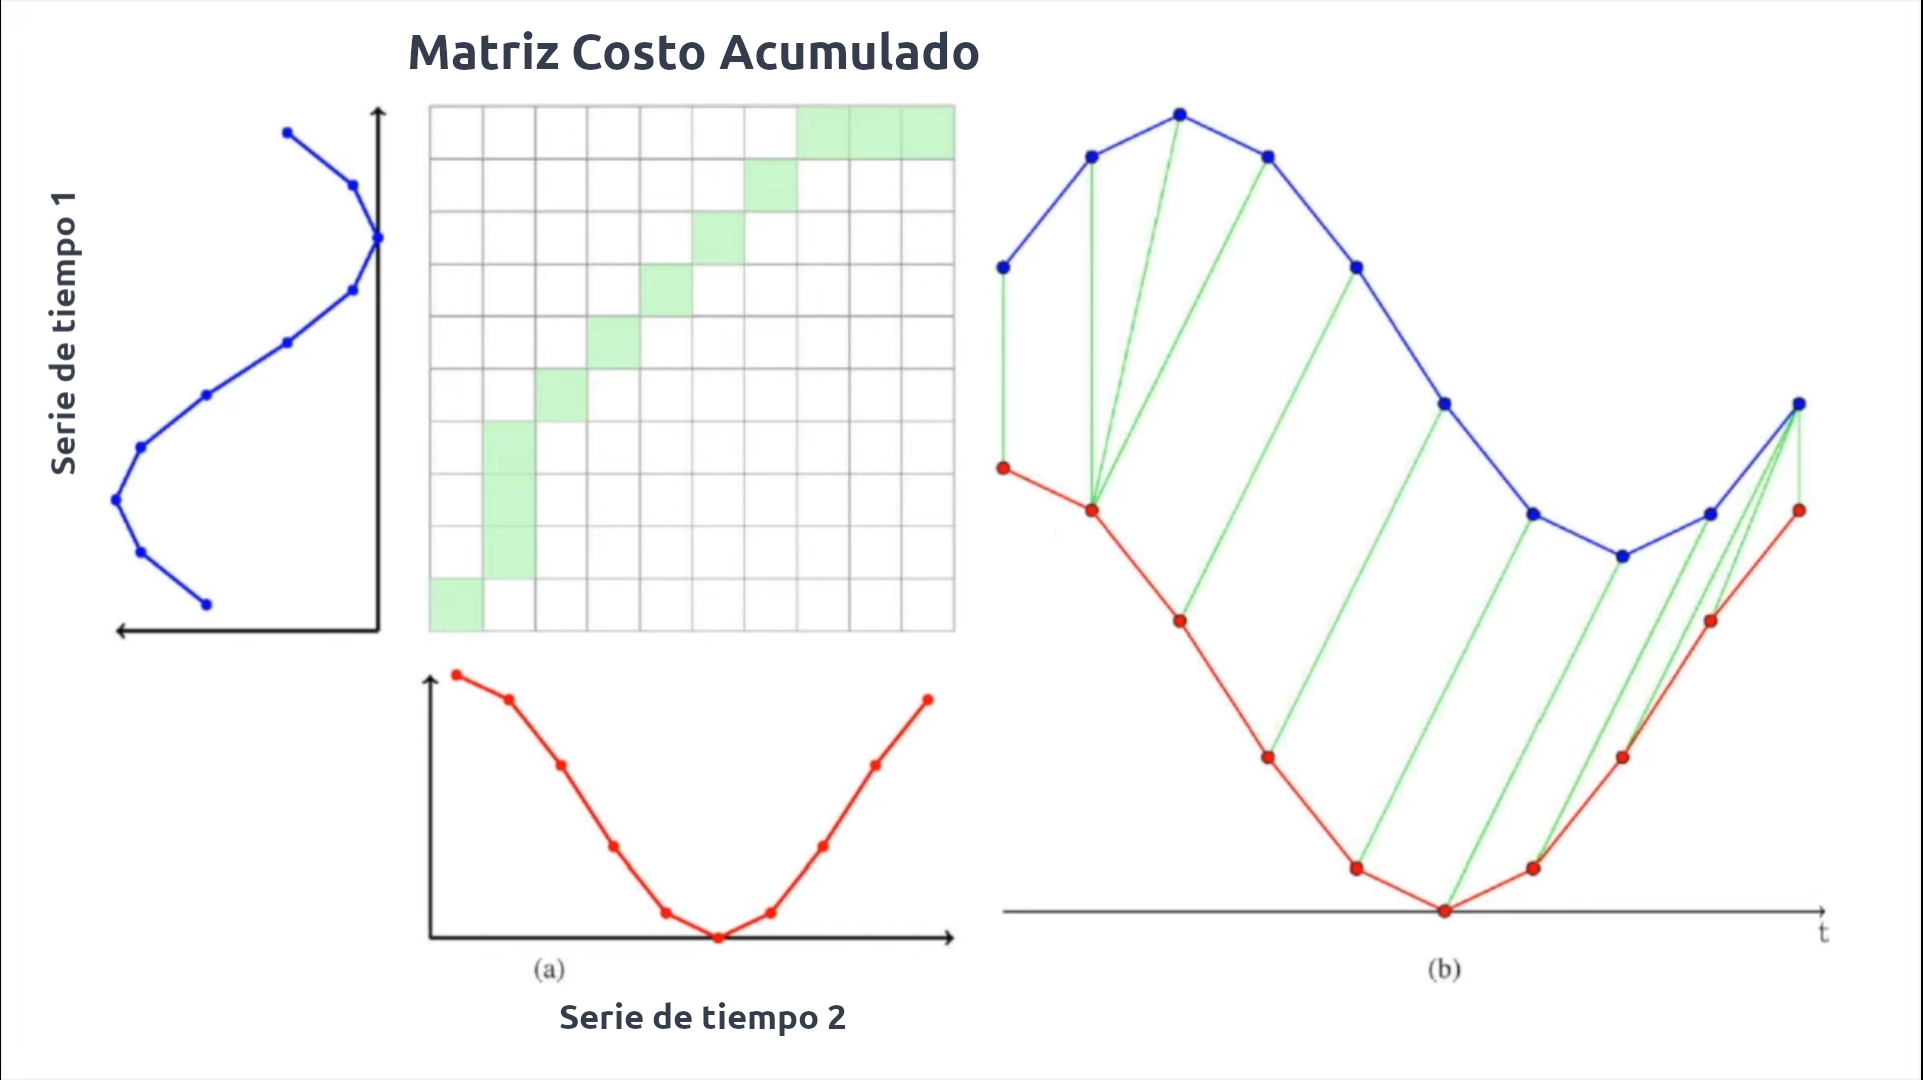
\includegraphics[width=\linewidth]{Imagenes/dtw.png}
		\label{dtw}
		\captionof{figure}{a) Matriz de costo acumulada del cálculo de la distancia entre la Serie de tiempo 1 y Serie de tiempo 2. Los recuadros verdes conforman el camino de deformación óptimo(\textit{optimal warping path}) $p^*$. \\b) Resultado de la alineación óptima para la Serie de tiempo 1 en la Serie de tiempo 2 utilizando DTW. \\{\small Figura recuperada de: Thales Sehn Körting(Productor).(2017) \textit{How DTW (Dynamic Time Warping) algorithm works}[YouTube]. https://www.youtube.com/watch?v=\_K1OsqCicBY}}
	\end{minipage}

\hfill\break
\justifying
\textbf{Banda Sakoe-Chiba}
	\hfill\break
	\justifying
	DTW es un algoritmo muy popular por sus excelentes resultados en la comparación de secuencias temporales, y sin embargo debido a la construcción de la matriz de costos, su complejidad cuadrática es un detractor significativo en tiempo y precisión de cálculo. Una variante común en DTW que aborda esta situación es la implementación de la banda Sakoe-Chiba[15].
	
	\hfill\break
	\justifying
	De forma general, la implementación de restricciones a DTW aporta un par de beneficios. El primero de ellos y el más importante si se plantea el objetivo de la optimización, es la reducción de complejidad con la implementación de la banda, forzando al cálculo de un subconjunto del espacio global e inmediatamente reduciendo su complejidad de $O(L^2)$ a $O(w\times L)$ con $0\geq w \leq L-1$, donde \textit{w} define una banda.
	
	\hfill\break
	\justifying
	El segundo de los beneficios refiere en cuanto a la fiabilidad de la similitud, pues previene alineaciones patológicas, evitando la desviación excesiva de la diagonal principal al camino óptimo posible.
	
	\hfill\break
	\justifying
	La banda Sakoe-Chiba corre a lo largo de la diagonal principal y tiene un ancho fijo $T \in \mathbb{N}$ horizontal y verticalmente(Figura 3). Esta restricción implica que para un elemento $x_n$ puede ser alineado únicamente a uno de los elementos de $y_m$ con $m \in \left[ \frac{M-T}{N-T} \times (n-T), \frac{M-T}{N-T} \times n+T \right] \cap [1:M]$. En la matriz de costo acumulado la ventana de deformación(\textit{warping window} o WW) se observa como en la Figura 3.
	
	\begin{minipage}{\linewidth}
		\centering
		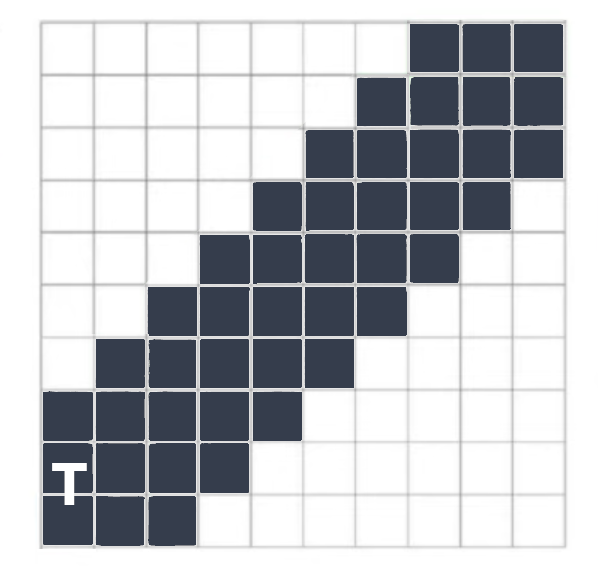
\includegraphics[width=6.5cm]{Imagenes/sakoe-chiba.png}
		\captionof{figure}{Banda de Sakoe-Chiba que corre sobre la diagonal principal de la matriz y que tiene un ancho fijo \textit{T}}
	\end{minipage}

\hfill\break
\justifying
\textbf{Optimización del tamaño de la ventana de DTW}
	\hfill\break
	\justifying
	El algoritmo DTW es un método robusto y con una extraordinaria competitividad, además de utilidad, probando ser una medida de distancia para series de tiempo excepcionalmente fuerte, y sin embargo parte de la comunidad subestima la capacidad del algoritmo por la ignorancia de lo importante que resulta la optimización del tamaño de la ventana \textit{w}, la cual es crítica en la disminución del error durante la predicción[16].
	
	\hfill\break
	\justifying
	Argumentando que la restricción en su cantidad máxima de deformación, cuando es establecida correctamente, cierra la mayoría de los espacios de mejora obtenidos con métodos de clasificación de series de tiempo ''más sofisticados'', el \textit{paper}[17] propone un método novel para el aprendizaje del parámetro óptimo en configuraciones supervisadas y no supervisadas, siendo el caso primero el que compete a este trabajo.
	
	\hfill\break
	\justifying
	Existe una concepción erronea del valor de \textit{w} dependiente del dominio de cálculo por única vez, cuando en realidad no existe un solo valor de \textit{w} que pueda ser transferible entre diferentes contextos, el valor óptimo para la banda restrictiva de DTW dependerá de 2 factores, el número de instancias del conjunto de datos y la estructura propia de los datos, contundentemente abatiendo la posibilidad de la existencia de un valor prototípico de \textit{w} para aplicaciones específicas como ritmos cardiacos o gestos[17].
	
	\hfill\break
	\justifying
	Formalmente el problema se plantea como: Dado un conjunto de entrenamiento de series de tiempo etiquetadas, encontrar el valor de \textit{w} que maximiza la calidad de clasificación en un conjunto de prueba sin etiquetar.
	
	\hfill\break
	\justifying
	La evaluación de la calidad de clasificación se realiza mediante la medida de la precisión.
	
	\hfill\break
	\justifying
	Debido al creciente consenso que ubica al método DTW-k-NN como una línea base robusta, deciden los autores del paper utilizar al algoritmo k-NN como el clasificador subyacente. Como se describe en secciones posteriores, este método es utilizado en todos los modelos evaluados, de forma que el clasificadores como k-NN y SVM son implementados también con diferencia al paper original.
	
	\hfill\break
	\justifying
	El enfoque que toma este método es particularmente útil cuando el conjunto de entrenamiento es limitado, pues implementa una técnica de remuestreo con la creación de datos sintéticos que remplazan al problema de un número de instancias limitadas.
	
	\hfill\break
	\justifying
	El algoritmo consiste en hacer \textit{N} copias del conjunto de entrenamiento original, remplazando para cada copia una fracción de los datos con remplazos sintéticos, para posteriormente realizar validación cruzada con el fin de aprender el porcentaje de error contra la curva de valores de \textit{w}. Se utiliza el valor promedio de todas las iteraciones \textit{N} para la predicción del mejor \textit{w}.
	
	\hfill\break
	\justifying
	De los componentes lógicos que conforman al método, los de mayor interés son el proceso de creación de un nuevo conjunto de datos con una porción sintética, y la función capaz de otorgar una deformación a una secuencia para otorgar un datos sintético.
	
	\hfill\break
	\justifying
	El proceso de creación de un nuevo conjunto de datos con instancias sintéticas inicia por dividir aleatoriamente el \textit{dataset} de datos, cumpliendo con una relación especificada de porcentaje de datos sintéticos sustitutos, permanece la otra partición sin modificación. Posteriormente utilizando k-Fold Cross Validation, se realiza la división en conjunto de entrenamiento y prueba para medir iterativamente la calidad del clasificador. 
	
	\hfill\break
	\justifying
	La función capaz de sintetizar una serie de tiempo inicia con el encogimiento no lineal de la medición real mediante la elimiación aleatoria de un porcentaje definido por el usuario, de los datos que la compone. Seguido a esto, utilizando una función común a bibliotecas de procesamiento de señales, la nueva serie debe remuestrearse a la misma longitud de la secuencia original, agregando antes de este proceso, un acolchado de la señal al repitiendo en los extremos los últimos y primeros 10 valores respectivamente. Finalmente y terminado el remuestreo, se eliminan los valores de acolchado en los extremos y se obtiene una serie sintética de longitud igual a la original.(Figura 4)
	
	\hfill\break
	\justifying
	Esta técnica requiere la configuración de 3 parámetros para su funcionamiento, utilizando como valores constantes para la experimentación los valores propuestos por los mismo autores del \textit{paper}, 20\% de deformación para la creación de datos sintéticos, una relación de 8 a 2 para la creación del nuevo \textit{dataset} con copias sintéticas como número de instancias mayoritarias, y finalmente el para número de iteraciones \textit{N}, mientras mayor sea su valor mejor, considerandose de forma conservativa en 10.  
	
	\begin{minipage}{\linewidth}
		\centering
		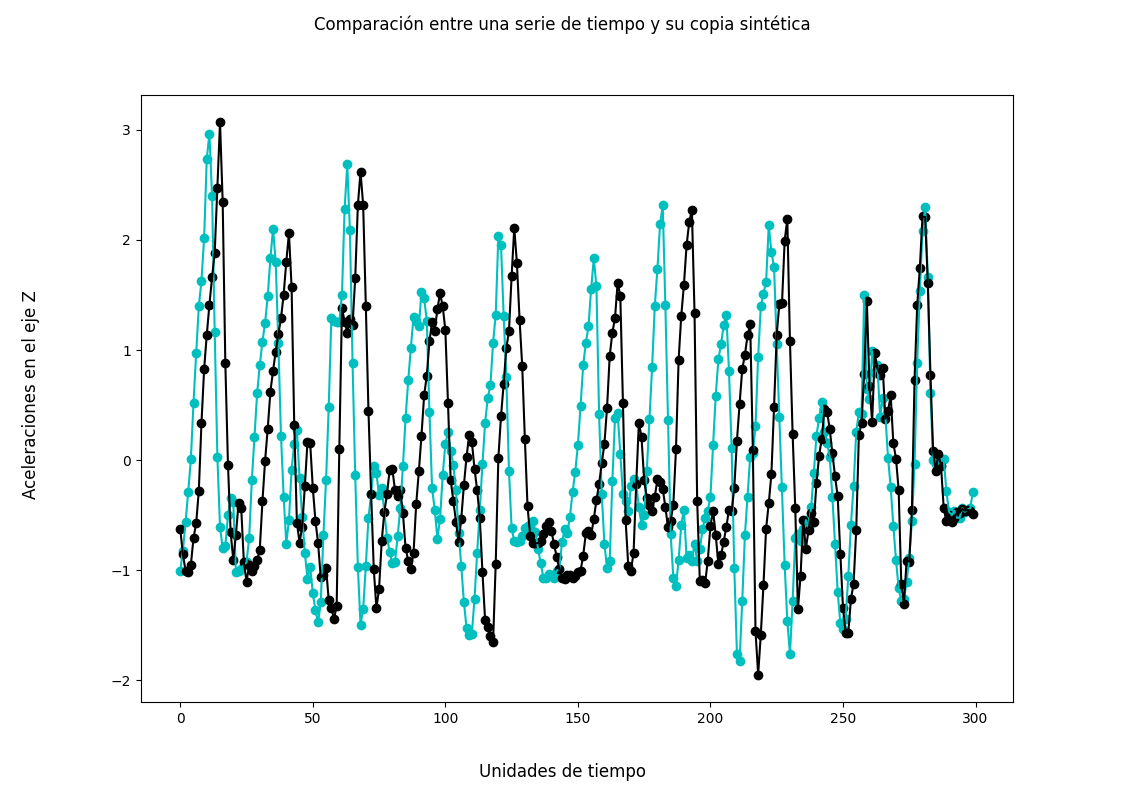
\includegraphics[width=9.5cm]{Imagenes/DTW_sinteticos_2.png}
		\captionof{figure}{Comparación de una instancia perteneciente al \textit{dataset} \textit{GesturePebble}(color azul) y su remplazo sintético(color negro)}
	\end{minipage}
\hfill\break
\justifying
\textbf{PAA}
	\hfill\break
	\justifying
	\textit{Piecewise Aggregate Approximation}(PPA) es un algoritmo que tiene como idea básica la reducción dimensional de una serie de tiempo de entrada mediante la partición de esta en segmentos del mismo tamaño, sobre cada cual se realiza el cálculo promedio de los valores en el segmento[18]. Con una serie de tiempo $Y = Y_1,Y_2,...,Y_n$ con tamaño $n \in \mathbb{R}$ la partición o reducción a una serie $X = X_1,X_2,...,X_m$ donde $m\leq n$, la ecuación que describe los elementos en la serie reducida es:
	
	\begin{equation*}
		\overline{X_i} = \frac{m}{n} \sum_{j=\frac{n}{N(i-1)+1}}^{\frac{n}{M}i}x_j
	\end{equation*}
	
	\hfill\break
	\justifying
	El aspecto más interesante del algoritmo es la forma en que se crean los segmento del mismo tamaño. Es importante notar que antes de realizar la aproximación promedio de cada ventana, el vector debe ser z-normalizado, y una vez haya sido estandarizado el vector la aproximación por partes se calcula.
	
	\hfill\break
	\justifying
	Identificados 2 casos escenciales durante la separación en segmentos. El caso trivial, $m<n$ y \textit{m} es múltiplo de \textit{n}, se trata dividiendo el vector en ventanas de tamaños iguales, sobre las que posteriormente se les realiza un cálculo del promedio para la asignación del nuevo valor a cada segmento. Por otra parte donde $m<n$ y \textit{m} no es múltiplo de \textit{n}, deja de existir un balance que evita la división exacta del vector en segmentos de mismo tamaño. Lo que ahora se requiere es que cada ventana sea redimensionada de forma que cada elemento de la serie de salida es el promedio de un segmento de mismo tamaño al vector de entrada[18].
	
	\hfill\break
	\justifying
	Se observa un ejemplo en la Figura 5 de la discretización de un par de series de tiempo con pocos atributos pero de extensión distinta, que despues de la transformación PAA son equiparables en longitud con un número de palabras \textit{m=9}.
	\begin{minipage}{\linewidth}
		\centering
		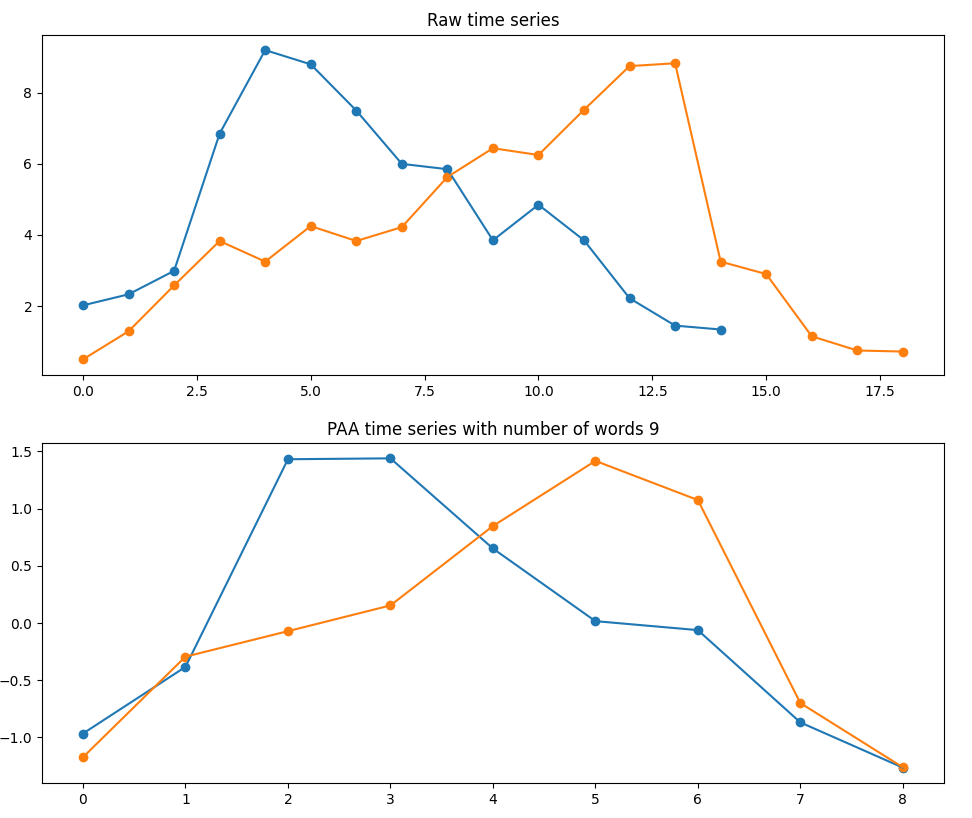
\includegraphics[width=\linewidth]{Imagenes/PAA.png}
		\captionof{figure}{Con el algoritmo PAA se mantienen las tendencias de las secuencias temporales, con la diferencia que han sido reducidos el número de valores que las conforman, nombradas palabras después de la discretización.}
	\end{minipage}
	
\hfill\break
\hfill\break
\justifying
\textbf{Symbolic Aggregate Approximation}
	\hfill\break
	\justifying
	SAX es una técnica desarrollada y enfocada en la reducción dimensional de una serie numérica con una serie de tiempo, a un espacio simbólico de 'palabras'. Dada una serie dependiente del tiempo de longitud arbitraria \textit{n} se realiza la transformación a una cadena de longitud \textit{w} utilizando un alfabeto $A={a_1,a_2,...,a_3}$[19].
	
	\hfill\break
	\justifying
	La primer parte de la discretización es manejada por la transformación PAA. siguiendole entoces el proceso de asignación de símbolos para cada sección, siendo requerimiento para esta segunda parte de la discretización, que los símbolos sean asignados equiprobablemente(propiedad de una colección de eventos teniendo la misma probabilidad de ocurrir). Esto se cumple facilmente por la previa normalización de los datos de la serie en una distribución Gausiana, por lo que las áreas bajo la curva de campana de la distribución pueden ser utilizadas para la creación de los puntos de quiebre(\textit{breakpoints}) en los datos normalizados para la asignación de palabras.
	
	\hfill\break
	\justifying
	El proceso del algoritmo toma los siguientes procesos en el siguiente orden[13]:
	\begin{enumerate}
		\item Estandarización o normalización-z de los datos de la serie de tiempo para tener una media de 0 y una desviación estándar de 1
		\item Transformación o reducción de dimensionalidad desde \textit{n} a \textit{w} mediante el algoritmo \textit{Piecewise Aggregation Approximation}(PAA)
		\item Asignación de los puntos de quiebre $\beta = \beta_1,...,\beta_{\alpha-1}$
		\item La serie de tiempo es discretizada tomando el promedio de cada segmento para ser mapeado a un alfabeto \textit{A}
	\end{enumerate}
	
	\hfill\break
	\justifying
	La distancia entre 2 Palabras o cadenas, correspondiendo cada una a diferentes series de tiempo, se calcula como el promedio de los pares de las distancias de símbolos.
	
	\hfill \break
	\textbf{Puntos de quiebre}
	\justifying
	Los puntos de quiebre es una lista de números $\beta = \beta_1,...,\beta_{\alpha - 1}$ tal que el área debajo la curva gausiana de $\beta_i$ a $\beta_{i+1}=\frac{1}{\alpha}$[19].
	
	\hfill\break
	\justifying
	Estos puntos de quiebre pueden ser obtenidos mirando una tabla estadística y puede ser utilizada para discretización de series de tiempo donde el coeficientes debajo el punto de quiebre más pequeño son mapeados a la letra del alfabeto en el índice 1, mientras los coeficientes mayores o igual al punto de quiebre más pequeño y menor al segundo punto de quiebre se le asigna la letra del alfabeto con el segundo ínidice, y así se sigue.
	
	\hfill \break
	\textbf{Distancia SAX}
	\justifying
	La distancia entre 2 símbolos se define a 0 si el índice difiere a lo más por 1(por ejemplo resulta 0 entre símbolos $a_i$ y $a_{i+1}$), en cualquier otro caso la distancia entre símbolos $a_i$ y $a_k$, donde $k>i$, se define como $b_{k-1}-b_i$[13].
	
	\hfill\break
	\justifying
	La distancia entre 2 cadenas correspondientes a diferentes series de tiempo, se calcula como el promedio de las distancias de los símbolos por parejas(por ejemplo; el promedio de la distancia entre el primer símbolo de cada serie, la distancia entre el segundo símbolo de cada serie, y así sucesivamente)[13].

\end{multicols}

\begin{figure}[!h]%
\begin{center}%
	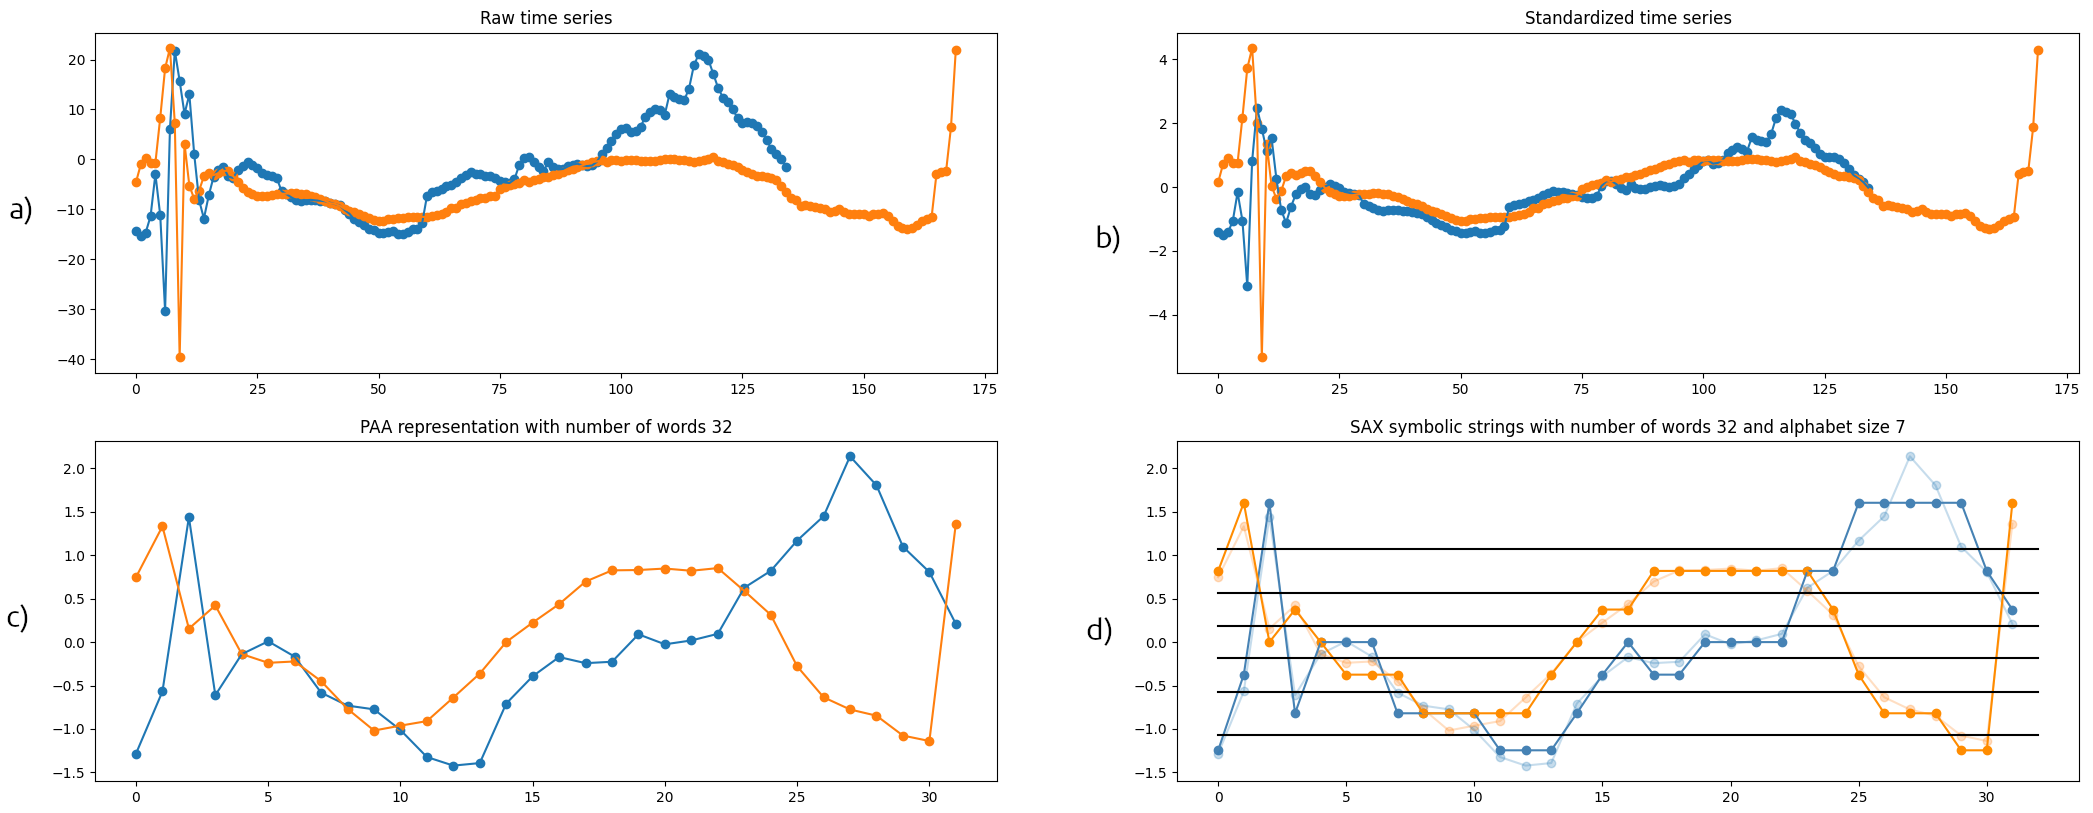
\includegraphics[width=\columnwidth]{Imagenes/SAX_example_2.png}%
	\caption{Graficación de un par de series de tiempo tomadas del \textit{dataset} \textit{GesturePebble} durante el proceso completo de la discretización SAX\\a) Series de tiempo de longitud variables con valores reales(originales)\\b) Series de tiempo después de estandarización.\\c) Series de tiempo después de la transformación PAA con un número de palabras igual a 32.\\d) Series de tiempo en su representación SAX como una cadena de símbolos numéricos con alfabeto de tamaño 7(En el fondo difuminadas se encuentra como referencia las mismas secuencias en representación PAA previo la discretización en símbolos de la cadena SAX).}
	\label{label}%
\end{center}%
\end{figure}%

\begin{multicols}{2}
\hfill\break
\justifying
\textbf{DTW Barycenter Averaging}
	\hfill\break
	\justifying
	\textit{DTW Barycenter Averaging}(DBA) es un algoritmo iterativo que utiliza DTW para la alineación de series de tiempo a ser promediadas con un promedio envolvente[20]. Introducido por Petitjean, la implementación del algoritmo DBA trae consigo varias ventajas importantes frente a un proceso plano o simple de promediación de un conjunto de secuencias.
	
	\hfill\break
	\justifying
	El algoritmo \textit{grosso modo}, opera de la siguiente manera:
	\begin{enumerate}
		\item Las \textit{n} series por ser promediadas son etiquetadas $S_1,S_2,...,S_n$ y tienen una longitud \textit{T}.
		\item Se inicia el proceso con una serie abreviada inicial \textit{A}.
		\item Mientras el promedio no haya convergido:
			\begin{enumerate}
				\item Por cada serie \textit{S}, se aplica DTW contra \textit{A} y se salva el camino de deformación.
				\item Se utiliza el camino de deformación y se construye un nuevo promedio de \textit{A} al dar a cada punto un nuevo valor: El promedio de cada punto de \textit{S} conectado a este en el camino de deformación resultante de DTW.
			\end{enumerate}
	\end{enumerate}

	\hfill\break
	\justifying
	Una buena inicialización del proceso con un candidato correcto para \textit{A}, es de extrema importancia, porque mientras el proceso DBA por si mismo es determinístico, el resultado final dependerá escencialmente on la secuencia abreviada inicial. Se identifican entonces 3 objetivos distintivos:
	\begin{itemize}
		\item Preservar la forma de las entradas.
		\item Preservar la magnitud de los extremos en el eje y.
		\item Preservar la sincronización de aquellos extremos en el eje x.
	\end{itemize}

	\hfill\break
	\justifying
	En el \textit{paper} se recomienda inicializar DBA eligiendo de forma aleatoria la serie abreviada de inicio \textit{A}, y en un principio esta técnica preserva bien la forma, pero la sincronización de los extremos dependerá en cual serie resulta escogida, razón por la que un proceso deterministico de elección es preferible.
	
	\hfill\break
	\justifying
	Una solución consiste en utilizar una serie de entrada para la inicialización, escogiendo mediante un proceso determinístico la entrada. Como primer paso de debe elimina la tendencia de cada una de las instancias en la serie, para paso seguido, guardar el valor en el eje x de los valores máximos y mínimos de cada serie. Finalmente la serie de inicialización abreviada, será la más cercana a la media de los valores guardados. Este proceso conserva la forma de las secuencias, las magnitudes extremas en el eje de las ordenadas, y finalmente obtener una noción clara de las posiciones típicas para x de aquellos extremos.
	
\end{multicols}

\hfill\break
\begin{figure}[!h]%
	\begin{center}%
		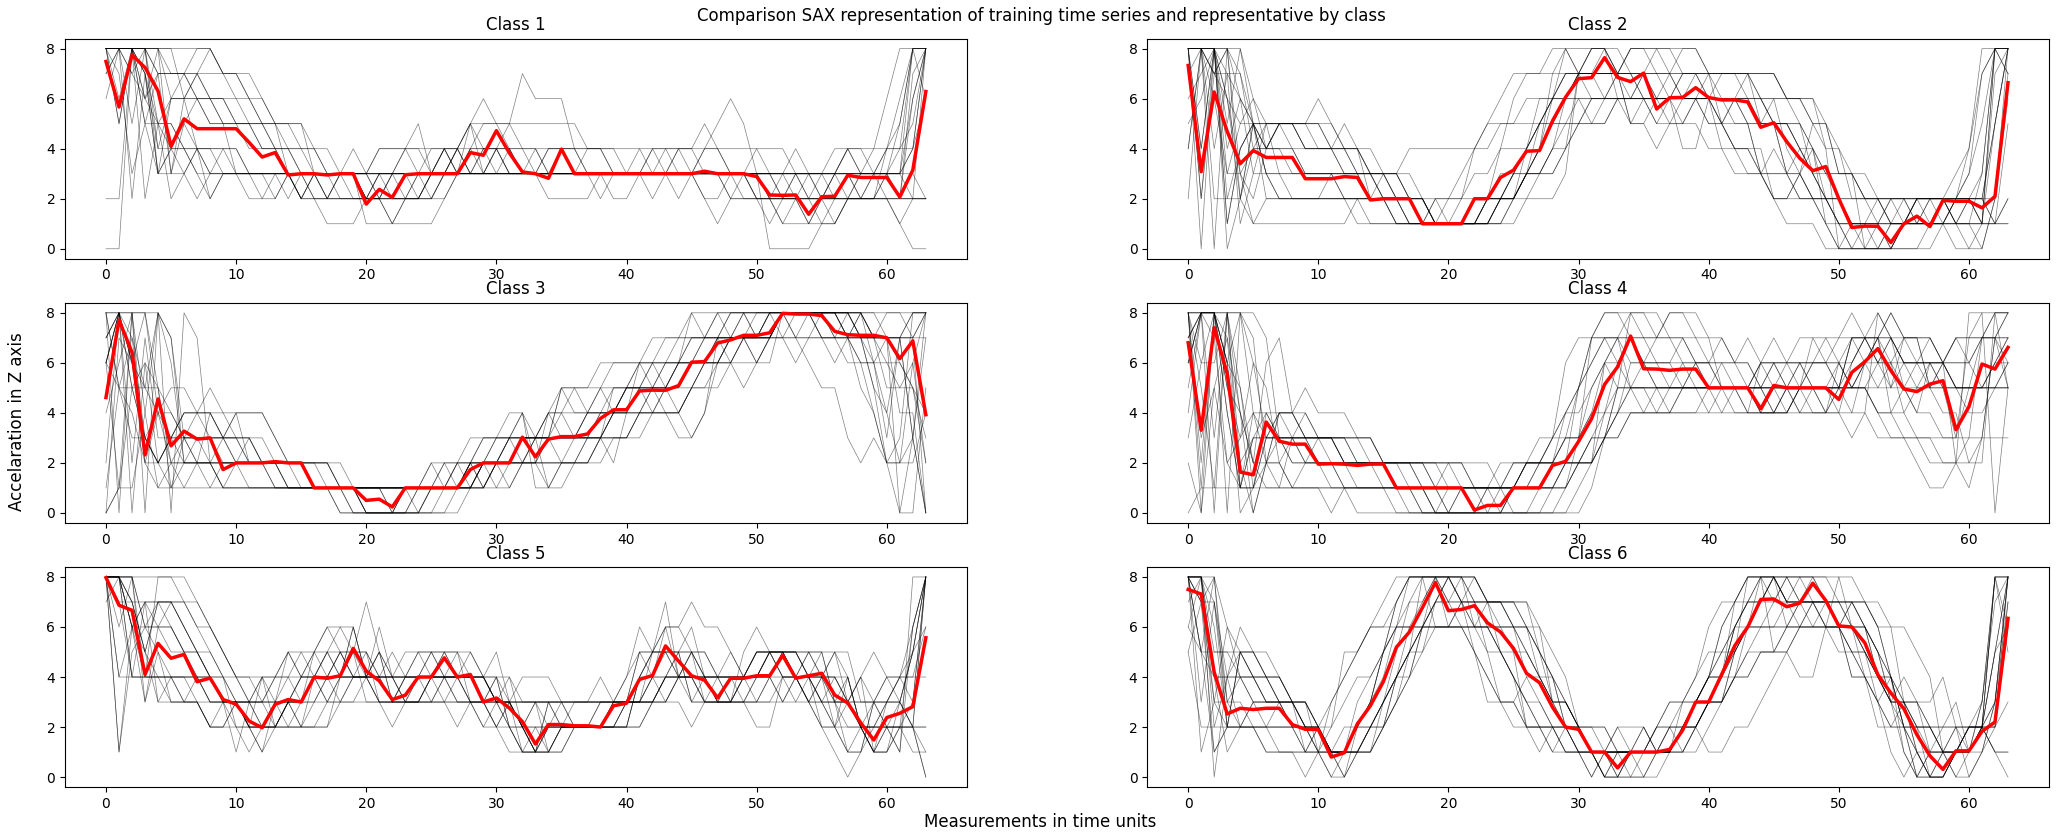
\includegraphics[width=\columnwidth]{Imagenes/DBA.png}%
		\caption{Ejemplo de las series representantes de cada clase para el conjunto de datos \textit{GesturePebble}. Cada representante(color rojo) fue calculada utilizando el algoritmo DBA con un promediado de 5 instancias discretizadas(color negro) en representación SAX de alfabeto tamaño 9 y número de palabras 64.}
	\end{center}%
\end{figure}%

\begin{multicols}{2}